% Activate the following line by filling in the right side. If for example the name of the root file is Main.tex, write
% "...root = Main.tex" if the chapter file is in the same directory, and "...root = ../Main.tex" if the chapter is in a subdirectory.
 
%!TEX root =  testMain.tex

\chapter[Robberies in ``real'' locations]{Robberies}


Why now go to a larger map, if we have already identified some problems? well, there can always be more problems :D 


New idea: A  larger, more interesting spatial situation. we know we can have agents walking around a simple flat simulation, but now we want a more life-like situation, a town, and they're going to rob shit.


\section{General information}
%  - investigating idioms with the Island Prior


Agent behavioural loop, etc. Look at the code its online.


\section{Experiment 1: General - can we create BNs of a robbery at Grote Markt?}

{\color{red} todo add complexity in simulation by adding simple evidence and add description of simulation}


\subsection{Introduction}
Here I talk about the Grote Markt and the more complex simulations that I created for it.

\subsection{Methods}

\begin{figure}[htbp]
\begin{center}
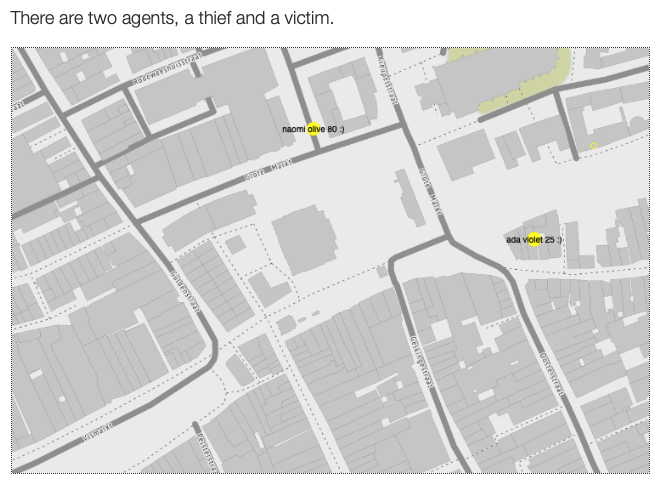
\includegraphics[width=\linewidth]{images/grotemarktmap.png}
\caption{map of environment - 2 agents}
\label{groteMarkt}
\end{center}
\end{figure}



\subsection{Results}

The network is shown in Figure~\ref{groteMarkperfo}.
\begin{figure}[htbp]
\begin{center}
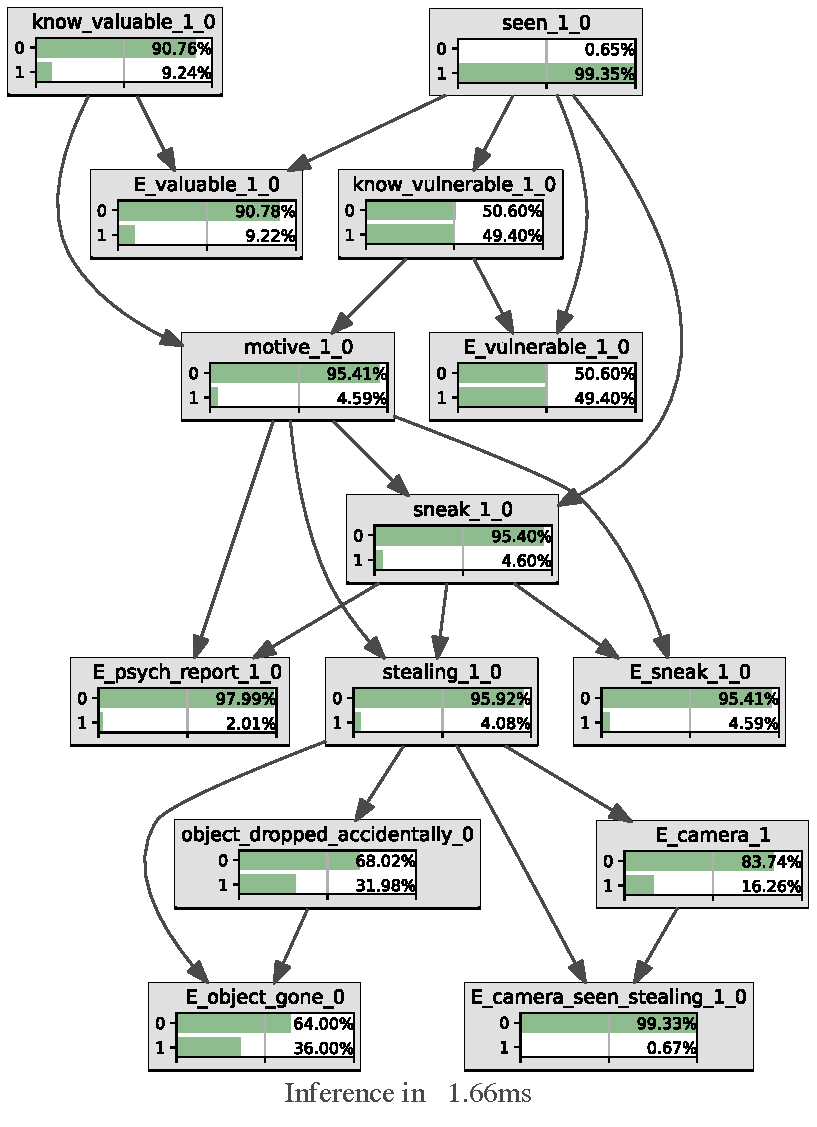
\includegraphics[width=.7\linewidth]{../experiments/GroteMarkt/bnImage/BNIMAGEGroteMarkt.pdf}
\caption{Bayesian NEtwork}
\label{groteMarktperfo}
\end{center}
\end{figure}

\subsection{Structural Criteria}
\begin{enumerate}
\item Hypotheses are ordered temporally. Following the cause-consequence idiom.
\item Evidence connects to hypotheses.
\item Relevance: All relevant events are in the BN, all irrelevant events are outside of the BN.
\item Independent events are not connected to each other.
\end{enumerate}

\subsection{Performance Criteria}
\begin{enumerate}
\item Accuracy.
\item Root Mean Squared Error.
\item Correspondence.
\item Sensitivity Values of Output Node.
\item Evidence updates the posterior in the correct direction.
\begin{figure}[htbp]
 \centering
%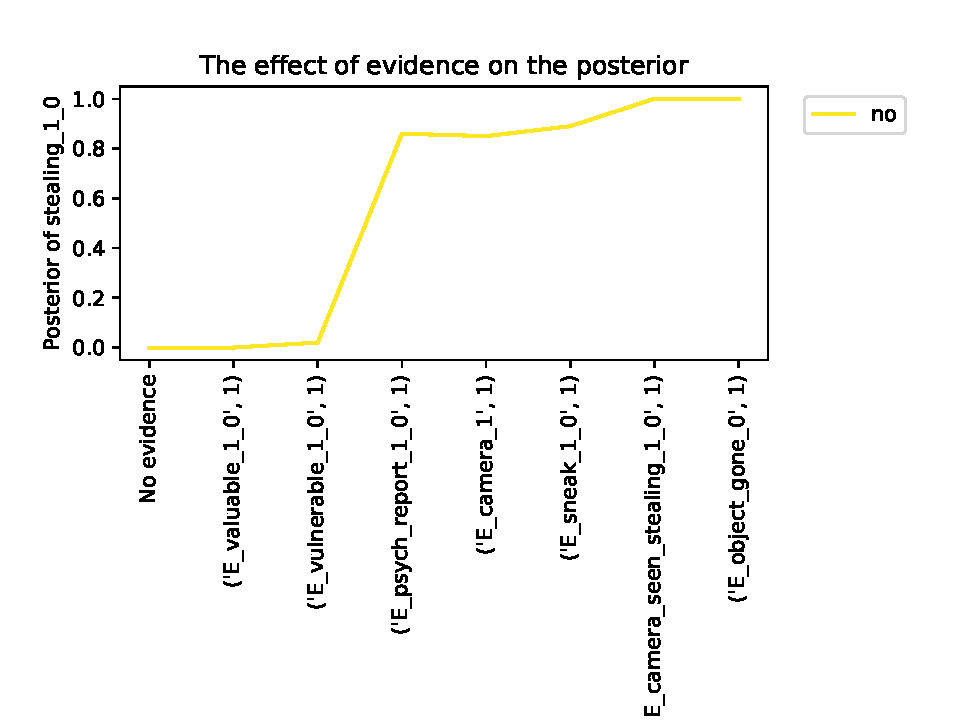
\includegraphics[width=0.6\linewidth]{../experiments/GroteMarkt/plots/posterior_base_networkGroteMarkt.pdf}
\caption{ Progression of evidence resulting in changing the posterior}
\label{baseposterior}
\end{figure}%
\end{enumerate}

\subsection{Human Criteria}
\begin{enumerate}
\item How robust is the network against a loss of precision?

\begin{figure}[htbp]
\begin{center}
\begin{subfigure}{.5\textwidth}
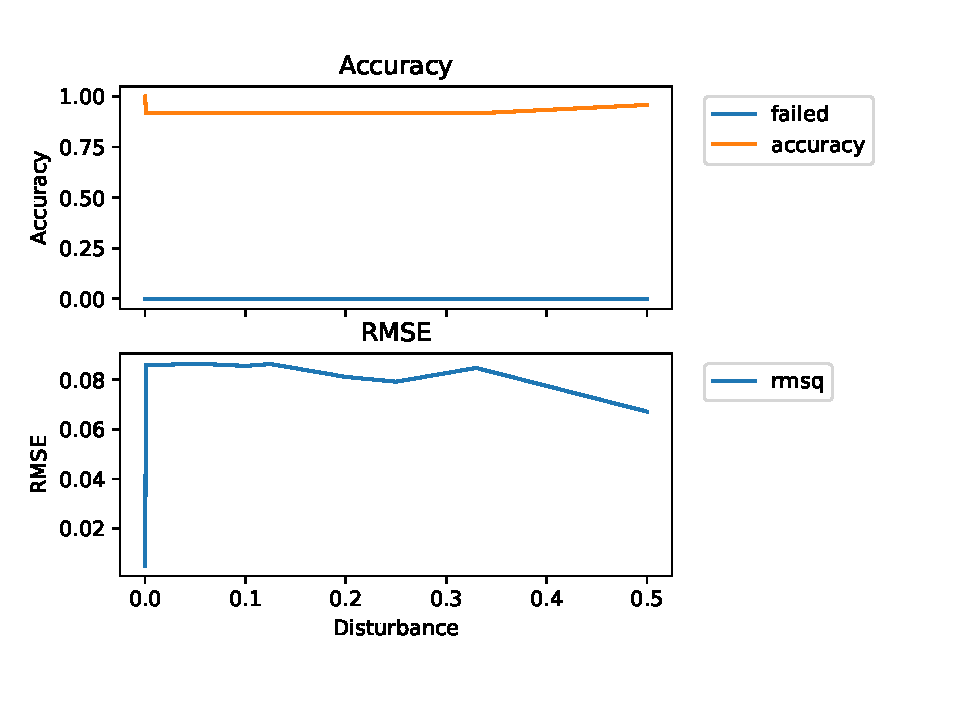
\includegraphics[width=0.9\linewidth]{../experiments/GroteMarkt/plots/performance_GroteMarkt.pdf}
\caption{Network Under Disturbance.}
\label{dist}
\end{subfigure}%
\begin{subfigure}{.5\textwidth}
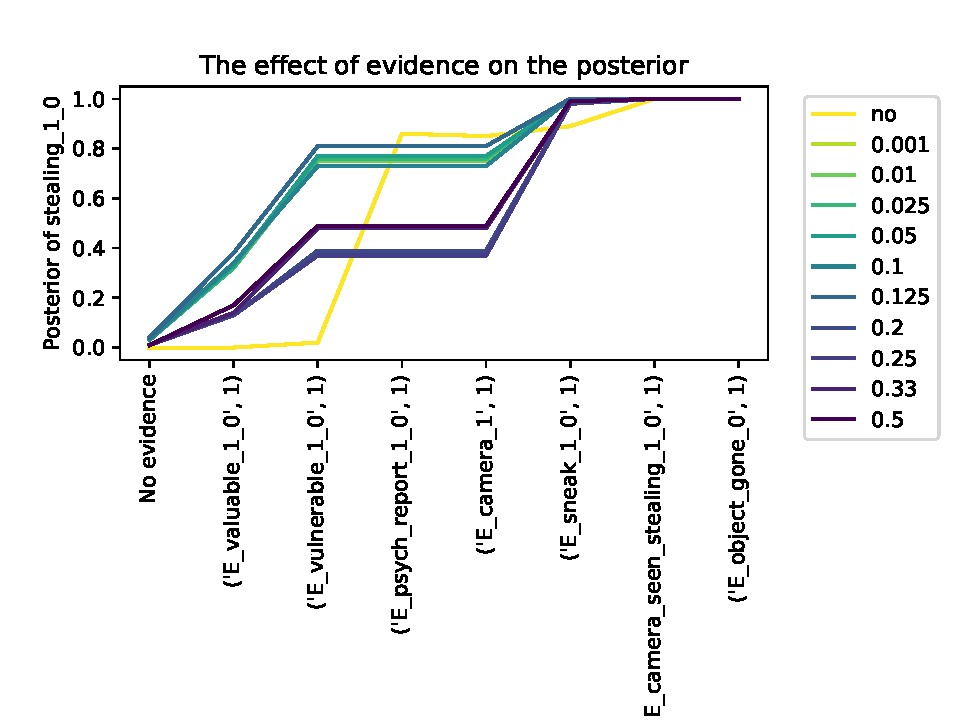
\includegraphics[width=0.9\linewidth]{../experiments/GroteMarkt/plots/posterior_GroteMarkt.pdf}
\caption{ Progression of evidence resulting in changing the posterior}
\label{post}
\end{subfigure}
\end{center}
\caption{Loss of precision in networks.}
\end{figure}

\item Could a human find these probabilities?
\item Can a human determine the correct independence relations?
\end{enumerate}

\subsection{Discussion}

\section{Experiment 2: Swapping out the maps.}
The geometry of the simulations that the agents move in is important. This means that we cannot just assume one prior for `seen'. This should be conditioned on the map.

\subsection{Introduction}
What happens if we have the exact same agent logic but we place them in a different spatial configuration? Instead of the Grote Markt, I now put some other part of Groningen in the simulation. We have the same nodes in the network. The only thing that's different is the underlying map.

I selected 5 different parts of Groningen, screenshotted then, converted them to maps like before, and then let the agents loose in them to rob each other.  Then I also made one part just completely empty, and one map random.

\subsection{Methods}

\subsubsection{Behaviour}
We keep the same behaviour as before (which is not described, sorry, ran out of time!).

\subsubsection{maps}
Image maps compilation in Figure~\ref{maps}.

\begin{figure}[htbp]
\begin{center}
\begin{subfigure}{.5\textwidth}
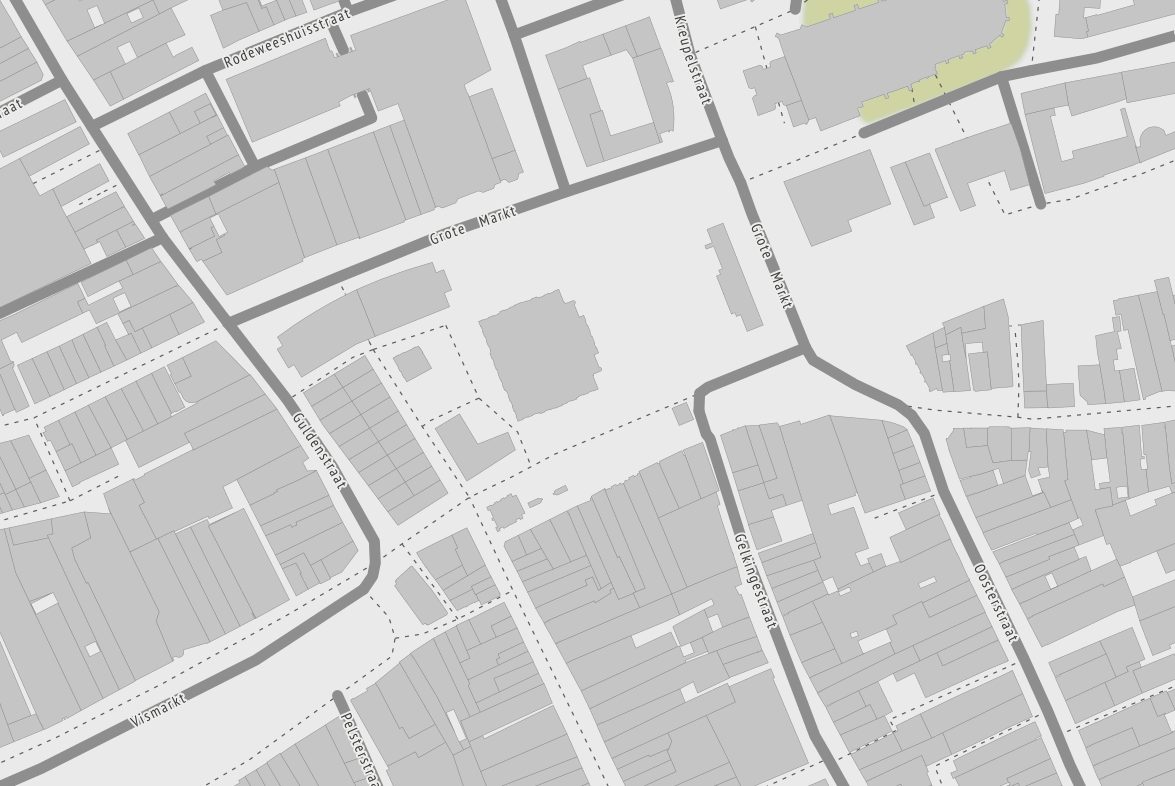
\includegraphics[width=0.8\linewidth]{../experiments/GroteMarktMaps/maps/groteMarkt.png}
\caption{Grote Markt.}
\end{subfigure}%
\begin{subfigure}{.5\textwidth}
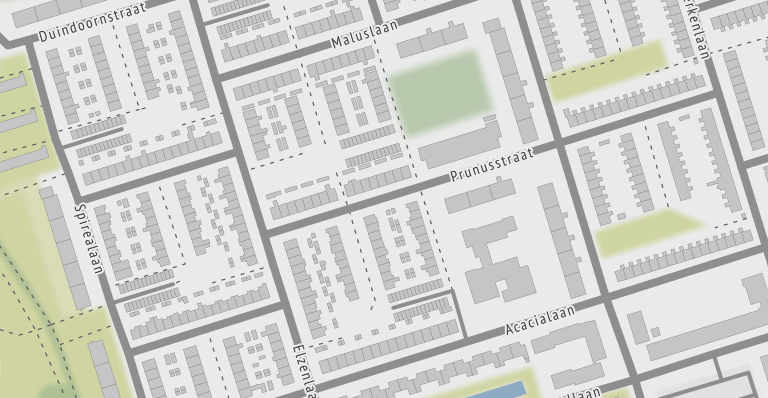
\includegraphics[width=0.8\linewidth]{../experiments/GroteMarktMaps/maps/Selwerd.png}
\caption{Selwerd.}
\end{subfigure}
\begin{subfigure}{.5\textwidth}
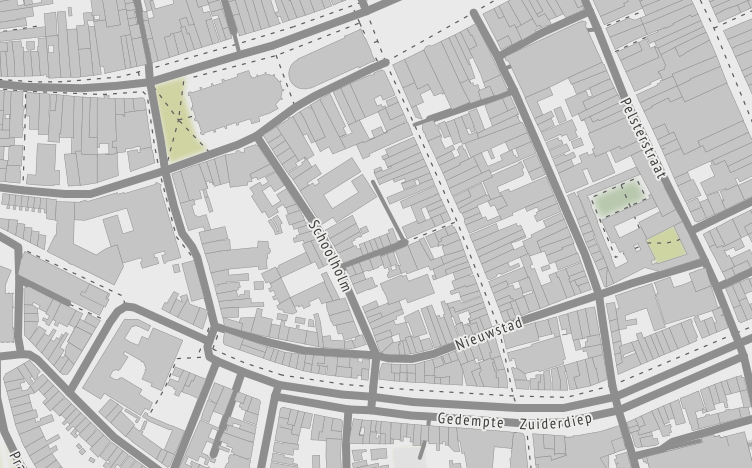
\includegraphics[width=0.8\linewidth]{../experiments/GroteMarktMaps/maps/zuidCentrum.png}
\caption{South-center}
\end{subfigure}%
\begin{subfigure}{.5\textwidth}
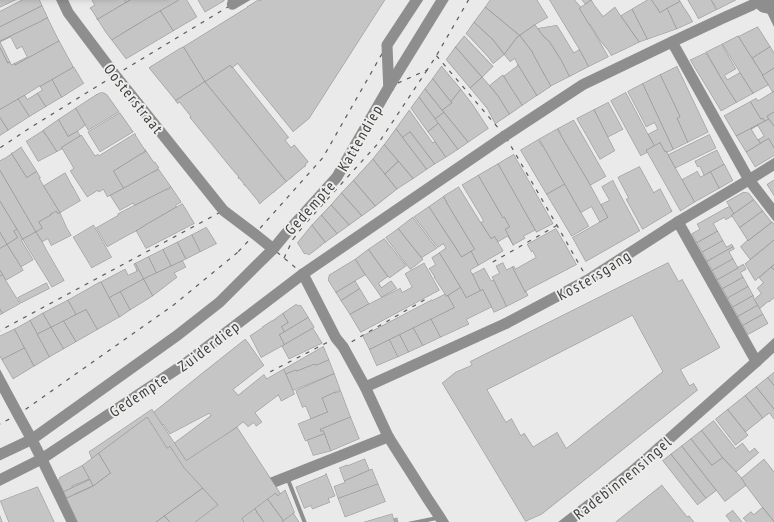
\includegraphics[width=0.8\linewidth]{../experiments/GroteMarktMaps/maps/kattediep.png}
\caption{Kattediep}
\end{subfigure}
\begin{subfigure}{.5\textwidth}
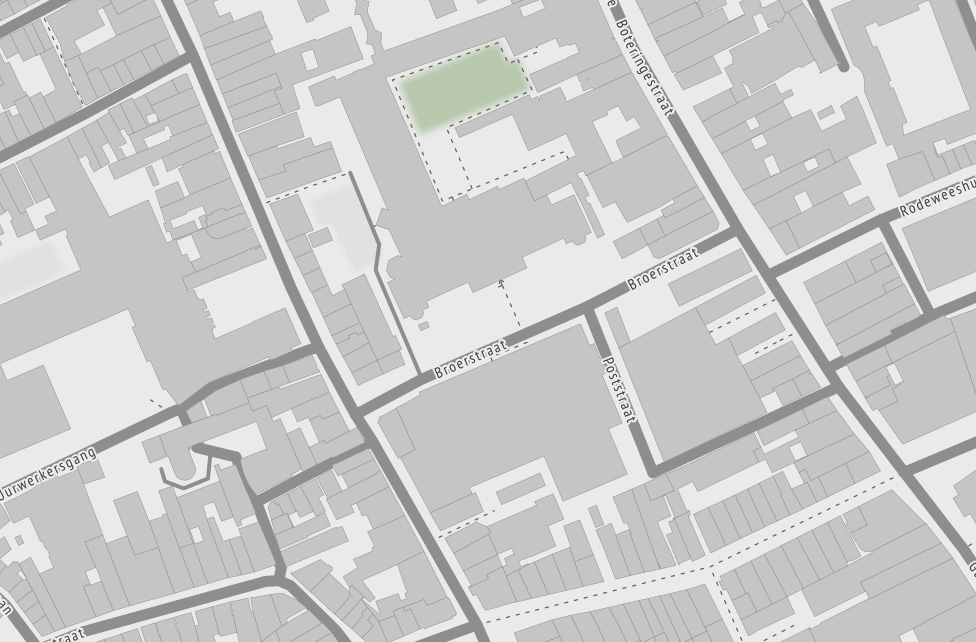
\includegraphics[width=0.8\linewidth]{../experiments/GroteMarktMaps/maps/academy.png}
\caption{Street with the academy building}
\end{subfigure}%
\begin{subfigure}{.5\textwidth}

\includegraphics[width=0.8\linewidth]{../experiments/GroteMarktMaps/maps/wall.png}
\caption{Not Groningen, just a wall}
\end{subfigure}
\caption{Maps.}
\label{maps}
\end{center}
\end{figure}


\subsection{Results}

We look at the difference in the cpt tables for `seen\_1\_0', which represents the event that agent 1 (the thief), sees agent 0 (Table~\ref{mapstab}). If we did not need to condition on underlying geometry of the simulation, we would expect that this probability would be the same, regardless of map. However, we find something different - the probability of the thief seeing the potential victim, depends on the underlying map, and not just `a bit', the smallest probability is 0.19 for the GroteMarkt map, while the largest is 0.50 for the Wall Map. At this difference, robustness to rounding does not hold!

This means that we actually cannot speak of just one `probability' for the agent seeing the victim - we can only speak of the probability of the agent seeing the victim, as conditioned on the map. 

\begin{table}[]
\begin{tabular}{lllll}
map & cpt of `seen\_1\_0' True \\
\hline
selwerd.png &0.26\\
academy.png & 0.47\\
groteMarkt.png  &0.19\\
kattediep.png &0.49\\
wall.png &0.50\\
zuidCentrum.png & 0.209\\
\end{tabular}
\caption{Difference in cpt depending only on difference in underlying map, no further difference in agent behaviour!}
\label{mapstab}
\end{table}

\subsection{Discussion}
Implications of this is that we need to condition explicitly on maps for our networks to work, because it does meaningfully change the probabilities that we find, and there's no way to predict how the map that we're using affects the probabilities. This has implications for the real world, because it means that we can't depend on some generic ``probability of getting robbed'', we need to condition on spatial conditions/background world assumptions.

And these are not even very good maps - agents can either go somewhere, or not. Affordances in the real world are very different \footnote{parkour!}. So it's likely that the actual probabilities in the real world are even worse...


\section{Discussion}
We have shown in this chapter that the specific geometry of simulation matters a lot for the results of the simulation. 

\subsection{Future Work}
The island prior.

